\chapter{Theoretical underpinning: Computer Supported Reflective
Learning}\label{csrl}

{[}Revision 4{]} - added figures

In order to inform the design of technology to support experiential
learning in crisis training, I adopted the Computer Supported Reflective
Learning model (hereafter CSRL model) developed by the MIRROR project.
The model identifies requirements to design technology to support
reflective learning \autocite{Krogstie:2013kf}. The CSRL model has
worked as theoretical underpinning for the development of applications
of technology presented in this PhD work, providing a language for
guiding the understanding of reflection and drafting requirements for
the technology.

After a brief introduction about theories in the field of reflective
learning, I describe the CSRL model and how it has been applied to the
development of technology. In the following I will use the terms
\emph{reflective learning} and \emph{reflection} as synonyms.

\section{Reflection as a tool for learning from
experiences}\label{reflection-as-a-tool-for-learning-from-experiences}

Boud \autocite*{boud1985reflection} defines reflective learning as ``a
generic term for those intellectual and affective activities in which
individuals {[}\ldots{}{]} explore their experiences in order to lead to
new understandings and appreciations'', it is both an individual and
collective mental process that turns past experiences into new
knowledge. This is also in line with the work of Schön
\autocite*{Schon:1983ut} who further distinguish between
\emph{reflection-in-action} and \emph{reflection-on-action}.

Reflection consists in a three-steps process during which the learner
re-evaluate her experiences inspecting behaviours, ideas and feelings;
eventually deriving conclusions and lessons learned to that guide future
behaviours (Figure \ref{fig:boud-model}). The process can be iterated
multiple times and might influence the learner behaviours only in the
long term.

\begin{figure}[htb]
    \centering
    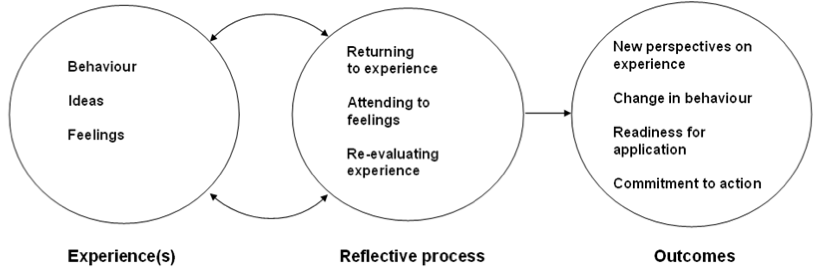
\includegraphics[width=1\textwidth]{boud}
    \caption{The reflection process according with Boud. Figure adapted from \protect\cite{boud1985reflection}}
    \label{fig:boud-model}
\end{figure}

A key aspect in making a reflective process to happen is the presence of
triggers. Triggers are unexpected situations, for example disturbances
and perception of uncertainty; but also positive situations like a
surprising success. In general, reflection seems to be triggered by
awareness of discrepancy between expectations and the current
experience. Reflection might be triggered by an external event or agent
(external trigger/accident) or might develop from one's own thinking of
a whole series of occurrences over time (internal trigger). Reflection
can occur incidentally or intentionally, but in both cases reflection is
a conscious evaluation of an experience. Furthermore people can learn
not only from their own experiences, but also from other's experiences
directly or indirectly (for example by observing and reflecting on
other's actions).

Similar to the work of Boud, Kolb describes experiential learning as a
cyclic process named ``The Kolb Cycle'' (Figure\ref{fig:kolb-model}).

\begin{figure}[htb]
    \centering
    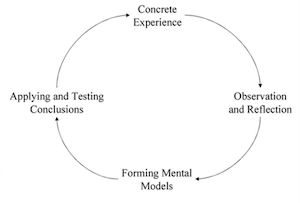
\includegraphics[width=1\textwidth]{kolb}
    \caption{"The kolb cycle", a model of experiential learning. Figure adapted from \protect\cite{kolb1984organizational}}
    \label{fig:kolb-model}
\end{figure}

According with Kolb \autocite*{kolb1984experiential} reflection is a
process that involves not only reinterpreting existing experiences, but
also initial perception and interpretation of the raw experience.

For a description of other existing theories in reflective learning see
\autocite{WoodDaudelin199636}.

\subsection{Debriefing crisis management work, an example of
collaborative
reflection}\label{debriefing-crisis-management-work-an-example-of-collaborative-reflection}

An example of collaborative reflection in crisis management is
\emph{debriefing}. As outlined by Boud et al.
\autocite*{boud1985reflection} debriefing is a form of collaborative
reflection because during debriefings a re-evaluation of experience
takes place, with explicit attention to emotions, ideas and behaviours.

Debriefing involves ``reviewing a difficult episode from a constructive
point of view \ldots{} the goal is to extract fundamental lessons
learned from the way the event was handled'' \autocite{Lagadec:1997js}.
It is a collaborative activity involving multiple roles and it is
usually performed after a (real or simulated) crisis work experiences.
Figure \ref{fig:debriefing-example} shows one of the debriefing observed
during the user studies reported in Chapter \ref{research}.

\begin{figure}[tbh]
    \centering
    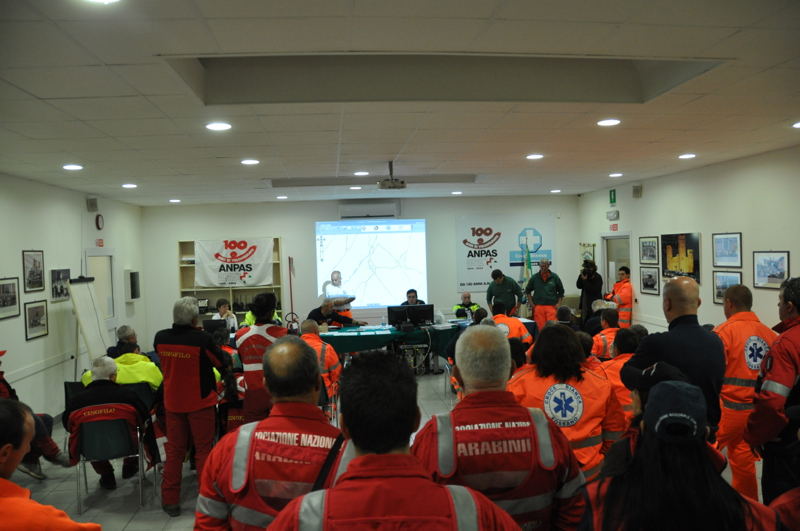
\includegraphics[width=1\textwidth]{debriefing}
    \caption{A debriefing after a physical simulation of crisis management attended by the author}
    \label{fig:debriefing-example}
\end{figure}

After a 3-days physical simulation of crisis management operations, the
chief manager discusses with team leaders and field workers what went
wrong and how to avoid the same issues in the future. Technology is used
to visualise location of operations on a digital map. Data were
previously manually entered during the training event.

The outcome which debriefing seeks to obtain is lesson drawing. Previous
work experiences provide a good source of lesson-drawing which may
potentially affect managing, planning and training for future crises.
Yet lessons-drawing is often one of the most neglected aspects of crisis
management \autocites{Lagadec:1997js}{Stern:1997eb}. The introduction of
debriefings into crisis organisations often meet resistance
\autocite{Lagadec:1997js}. This might be due to lack of commitment,
costs, but also the lack of technologies to make the debriefing more
effective.

\section{Computer Supported Reflective Learning, a
model}\label{computer-supported-reflective-learning-a-model}

Building on the presented theories and on empirical studies, the MIRROR
project has iteratively developed a model for Computer Supported
Reflective Learning (CSRL model). The model has been designed to
identify requirement, design and implement technology to support for
reflective learning \autocite{Krogstie:2013kf}. Rather than providing
formal guidelines or pre-defined processes, the model helps to
understand and analyse reflection in the workplace and it suggests how
technology can support reflective practicies.

Following the work of Boud et al. \autocite*{boud1985reflection} the
model considers reflective learning as ``the conscious re-evaluation of
experience for the purposes of guiding future behaviour {[}\ldots{}{]}
as reflection transforms experience from work into knowledge applicable
to the challenges of daily work'' \autocite{Krogstie:fo}. The model
specifically addresses reflection in the workplace with \emph{work} and
\emph{reflection on action} as loosely coupled activities that have an
impact on personal, collaborative and organisational growth. Therefore
the model is well suited to address reflection in the crisis domain in
which unexpected adverse events do not allow to schedule clear
boundaries between the time to be dedicated to work and to learning.

According with the model, a \emph{reflection session} is a time-limited
practice in which reflection happens. Reflection is driven by learning
objectives that might be only partially explicated, leaving rooms for
open-ended outcomes. Such outcomes may include a change in behaviour,
new perspectives and commitment for action
\autocite{boud1985reflection}. \emph{Participants} of the session might
be a single person (individual reflection) or multiple persons
(collaborative reflection).

The model explains reflective learning as a cycle involving fours stages
of reflection: (i) do work; (ii) initiate reflection session; (iii)
conduct reflection session; and (iv) apply reflection outcomes. For each
stage the framework specifies relevant sub-steps: specific
reflection-useful activities that can be augmented with technology. For
example, initiate reflection session includes \emph{decide to reflect}
and \emph{frame the reflection session}.

\begin{figure}[tbh]
    \centering
    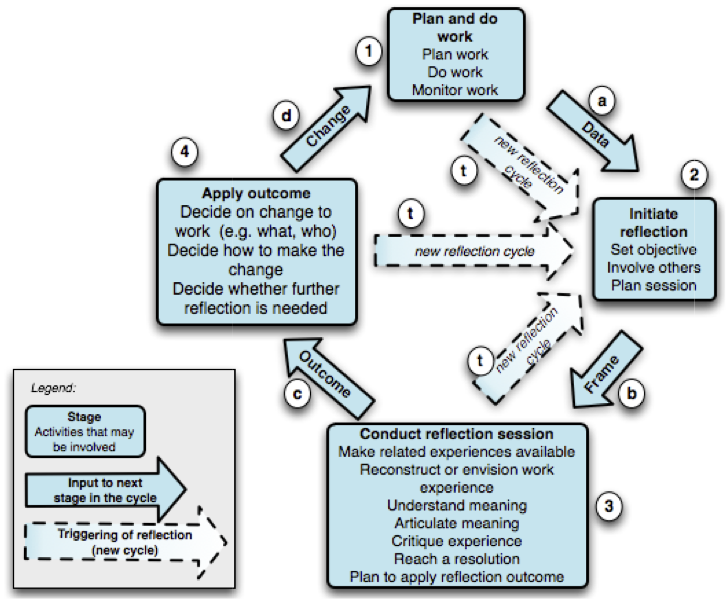
\includegraphics[width=1\textwidth]{CSRL}
    \caption{CSRL reflection cycle. Figure adapted from \protect\cite{Krogstie:2013kf}}
    \label{fig:csrl-model}
\end{figure}

Figure \ref{fig:csrl-model} depicts the models in terms of
\emph{stages}, \emph{inputs} and \emph{triggers}.

A \emph{stage} includes sub-activities that can be supported with
technology, \emph{inputs} are either raw or more or less contextualised
data being exchanged among stages; \emph{triggers} are either external
events or internal mental processes that initiate a reflection session.
Reflection can be triggered during work, while a change is about to be
applied or during the reflection session itself. In general, reflection
seems to be triggered by awareness of discrepancy between expectations
and the current experience.

Triggers also allow for including more actors in the reflection process,
iteratively starting new cycles based on the results of previous ones.
For instance, the outcome of a personal consideration (e.g.~how a crisis
procedure is applied) might be brought in a team meeting to trigger
collaborative reflection ultimately leading to a change in protocols. In
this way, we can look at reflection as a storyline that might involve
different actors within the organisation \autocite{PrPK13}.

\section{CSRL applied to the design of technology for crisis
training}\label{csrl-applied-to-the-design-of-technology-for-crisis-training}

The CSRL model can be used by designers to choose which technology to
use to support reflection activities or do derive requirements for the
design of new technologies \autocite{Krogstie:2013kf}.

For each stage, the CSRL model identifies support that can be provided
through technology. For example in the \emph{do work} phase, technology
could be used to monitor work and collect data that can be useful for
reflection, in \emph{initiate reflection} to set the objectives for
reflection or to involve others in the session, in \emph{conduct
reflection} to share work experiences with colleagues; and in
\emph{apply reflection outcomes} to decide how the change to work will
be implemented.

The model has driven the development of several software and hardware
applications within the MIRROR project; to address reflective learning
in the fields of social care, health care, business and emergency aid.
For a description of the applications see \autocite{Schwantzer:2014we}.
Several works \autocites{Krogstie:2013kf}{Krogstie:fo}{Krogstie:2012ki}
have shown how the four stages in the model can me mapped against
technologies to support individual and collaborative reflection.

In the case of crisis training I identified that the mapping between the
activities described by the CSRL model and technology can be placed into
three area (Figure \ref{fig:model-instantiation}):

\begin{itemize}
\itemsep1pt\parskip0pt\parsep0pt
\item
  technology to \textbf{capture} work experiences (for example by means
  of automatic sensors, a personal diary application, or a timeline
  visualisation)
\item
  technology to \textbf{re-create} work experiences, making use of the
  captured data to trigger and assist a reflection session with relevant
  information (for example by allowing to re-evaluate a past experiences
  from multiple point of views, in a context that help making sense
  processes during debriefing)
\item
  technology to \textbf{generate} new, realistic work experiences for
  training purposes (for example via virtual worlds, serious games, or
  tabletop exercises)
\end{itemize}

\begin{figure}[htb]
    \centering
    \includegraphics[width=1\textwidth]{model-instantiation}
    \caption{Instantiation of the CSRL model to support crisis training}
    \label{fig:model-instantiation}
\end{figure}

The three areas have in common the need for innovative interfaces
between people and technology. Yet the design of such user interfaces
aims at different goals. During \emph{capturing} the interface should
allow the capture of a variety of quantitative data and user-submitted
information without interrupting crisis work. The stage of
\emph{re-creating} experiences need tools for data visualisation and
manipulation capable to re-create a work experiences in a context that
promote reflection. Finally \emph{generating} experiences needs
interfaces to bring realism and engagement of real crises into a
simulated environment. Notably, the \emph{capture} of experiences is
done during the crisis work, which is subject to strict protocols that
limit the design space for the technology.

In the following chapter I will investigate how recent advances in the
field of sensing-based interaction can provide theoretical tools from
human-computer interaction theory for the design of user interfaces for
capturing, re-creating and generating crisis work experiences.
